\section{Teorema de la alternativa de Gordan. Reformulaciones.}
\newcommand{\ttt}{\textbf{\emph{t}}}
\newcommand{\sss}{\textbf{\emph{s}}}
\newcommand{\xx}{\textbf{\emph{x}}}
\newcommand{\yy}{\textbf{\emph{y}}}
\newcommand{\vv}{\textbf{\emph{v}}}
\newcommand{\ww}{\textbf{\emph{w}}}
\newcommand{\zz}{\textbf{\emph{z}}}
\newcommand{\ccc}{\textbf{\emph{c}}}

Una vez que disponemos de la herramienta fundamental, el teorema de Mazur-Orlicz-König, nos disponemos a dar una versión convexa del teorema de la alternativa de Gordan. Antes de ello, y haciendo uso de este teorema tipo Hahn-Banach, probaremos el lema de Simons, sobre cierta condición de optimalidad para funciones convexas. \\

Antes de comenzar, necesitamos hacer la siguiente definición. Para agilizar la lectura, cuando indicamos $ N\in \NN $ estamos suponiendo que $ N \geq 1 $. También, para $ N \in \NN $, notaremos con caracteres en negrita a los elementos de $ \RR^N $, por ejemplo, $  \ttt = (t_1,...,t_N)\in \RR^N$. 

\begin{definicion}
	Dado $ N \in \NN $ llamamos símplex unitario de $ \RR^N $ al subconjunto de $ \RR^N $ definido como:
	\begin{equation*}
	\Delta_N := \left\lbrace \ttt \in \RR^N: \sum_{i=1}^{N}{t_i} = 1, \hspace{0.5em} t_1,...,t_N \geq 0 \right\rbrace .
	\end{equation*}
\end{definicion}

Recordamos ahora la noción de envolvente convexa de un subconjunto cualquiera $ X $ de un espacio vectorial $ \vecSpace $, que notamos como $ \mathrm{co}(X) $ y que se define como la intersección de todos los conjuntos convexos que contienen a $ X $. Nótese que $ \Delta_N = \mathrm{co}\{e_1,...e_N\} $. \\

Antes de continuar veamos que $ \Delta_N $ es convexo y compacto:

\begin{itemize}
	\item  Convexo: tenemos que comprobar que dados $ \ttt, \sss \in \Delta_N \text{ y } \lambda \in \lbrack 0,1 \rbrack $ entonces $ \lambda\ttt + (1-\lambda)\sss \in \Delta_N $. En efecto, las coordenadas $ \lambda t_i + (1-\lambda)s_i $ verifican:
	\begin{itemize}
		\item [i) ] $ \lambda t_i + (1-\lambda)s_i \geq 0 $ para todo $ i = 1,..., N $, ya que $ t_i, s_i \geq 0 $ y $ 0 \leq \lambda \leq 1 $.
		\item [ii) ] 
		\begin{equation*}
		\begin{split}
		\sum_{i=1}^{N} (\lambda t_i + (1-\lambda)s_i) &=   \lambda \sum_{i=1}^{N} t_i + (1-\lambda)\sum_{i=1}^{N} s_i \\
		&= \lambda + (1 - \lambda) \\ &= 1,
		\end{split}
		\end{equation*}ya que $ \sum_{i=1}^{N} t_i = \sum_{i=1}^{N} s_i = 1  $.
	\end{itemize}
	
	Por lo tanto, $ \lambda\ttt + (1-\lambda)\sss \in \Delta_N \text{ para todo }\lambda \in \lbrack 0,1 \rbrack $.
	
	\item Compacto: al encontrarnos en $ \RR^N $ y aplicando el conocido Teorema de Heine-Borel basta y sobra ver que $ \Delta_N $ es cerrado y acotado. Pero claramente es acotado por lo que nos centraremos en probar que es cerrado. Sea $ \lbrace \ttt_n \rbrace_{ n \in \NN} $ una sucesión de $ \Delta_N $ y sea $ \ttt_0 \in \RR^N $ tal que $ \lbrace \ttt_n \rbrace_{ n \in \NN} \longrightarrow \ttt_0 $. Tenemos que comprobar que $ \ttt_0 \in \Delta_N $. 
	\begin{itemize}
		\item[i) ] Como todas las coordenadas de cada $ \ttt_n $ para $ n \in \NN $ son no negativas las de $ \ttt_0 $ también lo son.
		\item[ii) ] La función $ f: \RR^N \longrightarrow \RR $ definida como $ f(\ttt) =  \sum_{i=1}^{N} t_i $ es continua. Claramente $ f(\ttt) = 1 $ para todo $ \ttt \in \Delta_N $ y por ello $ \lbrace f(\ttt_n) \rbrace_{ n \in \NN} \longrightarrow 1$. Por continuidad de $ f $ y unicidad de límite tenemos que $ f(\ttt_0) = 1 $ pero eso equivale a que la suma de sus componentes vale 1.
	\end{itemize} 
	
	Así, hemos demostrado que $ \ttt_0 \in \Delta_N $ y por lo tanto $ \Delta_N $ es compacto. 
\end{itemize}


\paragraph{}Antes de continuar, notamos que el espacio vectorial de todas las aplicaciones lineales de $ \RR^N $ a $ \RR $, con $ N \in \NN $, se puede identificar con $ \RR^N $. Esto se debe a que si $ L:\RR^N \longrightarrow \RR $ es lineal, entonces es de la forma $ L(\xx) = a_1x_1 + \cdots + a_Nx_N $, que se corresponde con $ \textbf{\emph{a}} = (a_1,\dots,a_N) \in \RR^N $. Del mismo modo, dado el vector tenemos la aplicación lineal asociada. En definitiva, el espacio dual de 
$ \RR^N $ se identifica con $ \RR^N $ .
\paragraph{} También presentamos el producto escalar usual en $ \RR^N $ que definimos como:
\[
\begin{split}
\langle \cdot, \cdot \rangle : \RR^N \times \RR^N \longrightarrow &\RR \\
(\xx, \yy) \longmapsto &\langle \xx, \yy \rangle = \sum_{i=1}^{N}x_iy_i.
\end{split}
\]

Antes de enunciar el lema de Simons, hacemos otra identificación, esta vez, correspondiente a un símplex unitario:
\bigskip
\begin{lemaBox}\label{lema2.1}
	Sea $ N \in \NN $ y $ S: \RR^N \longrightarrow \RR $ definida por: \[ S(\xx):=\max\{x_1,...,x_N\}.\] Entonces, $ S $ es sublineal. Además, si $ L:\RR^N \longrightarrow \RR $ es un funcional lineal tal que $ L \leq S $ entonces $ L $ es de la forma \[ L(\xx) = t_1 x_1 + ... + t_N x_N \] con $ (t_1,...,t_N) \in \Delta_N$. De hecho, el recíproco también es cierto, es decir, si $ L = \ttt = (t_1,...,t_N) \in \Delta_N $ entonces $ L \leq S $.
	
	%%%%%% NOTA %%%%%%%%
	%% Las aplicaciones lineales coninciden con el dual del espacio. Es decir, podemos identificar la aplicación con sus coeficientes obeniendo de ese modo un punto del espacio.
	
\end{lemaBox}
\begin{proof}
	Claramente, $ S $ es positivamente homogénea. También es sub\-aditiva ya que dados $ x,y \in \vecSpace $ : 
	\begin{equation*}
	\begin{split}
	S(\xx+\yy) &= \max \{x_1 + y_1, ..., x_N +y_N \}\\ 
	&\leq \max\{x_1, ..., x_N\} + \max \{y_1, ...,y_N\} = S(\xx) + S(\yy).
	\end{split}
	\end{equation*}
	
	Por ello, $ S $ es sublineal. Para terminar veamos que  \[\left\lbrace L:\RR^N \longrightarrow \RR : L \text{ lineal y }L\leq S \right\rbrace  =  \Delta_N \]
	a través de la correspondencia mostrada anteriormente entre $ \RR^N $ y su dual.
	
	\begin{itemize}
		\item[$ \supseteq $ )] Sea $ \mathbf{t} \in \Delta_N$, definimos $ L:\RR^N \longrightarrow \RR $ como $ L(\xx):= \langle \mathbf{t},\xx \rangle $. Es evidente que $ L $ es lineal en $ \xx $ al ser el producto escalar bilineal. Dado $ \xx \in \RR^N $,
		\begin{equation*}
		L(\xx) = \sum_{i=1}^{N}{t_i x_i} \leq \sum_{i=1}^{N}{t_i S(\xx)} = S(\xx)\sum_{i=1}^{N}{t_i} = S(\xx),
		\end{equation*}
		donde la primera desigualdad se debe a que $ x_i \leq S(\xx)$ para todo $ x_i$ con $ i=1,...,N $ y a que $ t_i \geq 0 $ ya que $ \mathbf{t} \in \Delta_N$. Esto también justifica la última igualdad ya que $ \sum_{i=1}^{N}{t_i} = 1 $.
		
		\item[$ \subseteq $ )] Sea $ L = \ttt = (t_1,...,t_N) \in \RR^N $ lineal tal que para todo $ \xx \in \RR^N $ cumple que $ \sum_{i=1}^{N}{t_i x_i} \leq S(\xx)$. Así, si tomamos $ e_i \in \RR^N $ donde $ e_i $ representa el i-ésimo elemento de la base usual de $ \RR^N $ con $ i=1,...,N $, entonces 		
		\begin{equation*}
		L(-e_i) = -t_i \leq 0 \Longrightarrow t_i \geq 0 \quad \forall i=1,...,N.
		\end{equation*}
		Si ahora llamamos $ e = \sum_{i=1}^{N}{e_i} $, obtenemos:
		\begin{equation*}
		\begin{rcases*}
		L(e) = \sum_{i=1}^{N}{t_i} \leq \max \{1, ...,1\} = 1 \\
		L(-e) = -\sum_{i=1}^{N}{t_i} \leq \max \{-1, ...,-1\} = -1
		\end{rcases*} \Longrightarrow \sum_{i=1}^{N}{t_i} = 1.
		\end{equation*}
		Concluimos entonces que $ L = \ttt = (t_1,...,t_N) \in \Delta_N $.
	\end{itemize}
	
\end{proof}
\bigskip

Enunciamos ahora el lema de Simons \cite{Simons2008}. Tal y como se ha mencionado antes, se trata de un resultado sobre funciones convexas y cierta condición de optimalidad: dos funciones distintas poseen el mismo ínfimo en un convexo. Esto sugiere el uso del teorema de Mazur-Orlicz-König.
\bigskip
\begin{lemaBox}[Simons]\label{Simons}
	Sea $ C $ un subconjunto convexo de un espacio vectorial y $ N \in \NN $. Dadas $  $ $ f_1, \dots, f_N : C \longrightarrow \RR $, funciones convexas, entones existe $ \ttt \in \Delta_N $ que cumple
	\[
	\inf_{c \in C}\left[ \max_{i=1\dots,N } f_i(c)\right] = \inf_{c \in C} \left[ \sum_{i=1}^{N} t_i f_i(c) \right].
	\] 
\end{lemaBox}
\begin{proof}
	Sea  $ \vecSpace = \RR^N $. Definimos $S:\hspace{1mm}\vecSpace \longrightarrow \RR $ como \[ S(x_1, ..., x_N) := \max \{x_1, ..., x_N\}. \] Por el lema \ref{lema2.1}, $ S $ es sublineal. Tomamos el subconjunto:
	\[ 
	D = \{ (x_1, ..., x_N)\in V: \exists c \in C \quad \text{ tal que } \quad \forall i = 1,...N,\quad f_i(c) \leq x_i \}.
	\]
	Comprobemos en primer lugar que $ D $ es un subconjunto convexo de $ \vecSpace $. Sean $ \xx, \yy \in D $, por ello, existen $ c_x, c_y \in C $ tales que $ f_i (c_x) \leq x_i  $ y $ f_i (c_y) \leq y_i \quad \forall i=1,...,N $. Dado $ \lambda \in [0,1] $, llamamos $ c := (1-\lambda)c_x + \lambda c_y $ que pertenece a $ C $ por ser este convexo. Veamos que $ c $ es el elemento necesario de $ C $ para que cualquier combinación convexa de $ x $ e $ y $ esté en $ D $. Así, para todo $ i =1,...,N  $:	
	\[
	f_i(c) = f_i((1-\lambda)c_x + \lambda c_y) \leq (1-\lambda)f(c_x) + \lambda f(c_y) \leq (1-\lambda)x_i + \lambda y_i ,
	\]
	donde la primera desigualdad se debe a que las $ f_i $ son convexas y la segunda a que $ \xx,\yy \in D $. Por ello, $ (1-\lambda)x_i + \lambda y_i \in D , \quad \forall \lambda \in [0,1] $ por lo que $ D $ es convexo. Aplicando el Teorema de Mazur-Orlizc-König, existe $ L $ funcional lineal en $ \vecSpace $ tal que $ L \leq S $ e $ \inf_D L = \inf_D S $. \\
	
	Nuevamente, por el lema \ref{lema2.1} tenemos que $ L = \ttt \in \Delta_N$. Finalmente:
	\[
	\inf_D L =\inf_{c \in C} \left[ \sum_{i=1}^{N} t_i f_i(c) \right]
	\]
	e
	\[
	\inf_D S = \inf_{c \in C}\left[ \max_{i=1\dots,N } f_i(c)\right]
	\]
	por lo que 
	\[ \inf_{c \in C}\left[ \max_{i=1\dots,N } f_i(c)\right] = \inf_{c \in C} \left[ \sum_{i=1}^{N} t_i f_i(c) \right]. \] 
\end{proof}
\bigskip
Enuciamos ahora el Teorema de la Alternativa de Gordan en su versión clásica.
\bigskip
\begin{teoremaBox}[Teorema de la alternativa de Gordan]\label{GordanClasic}
	Dados $N, M \in \NN   $, sean $ \{\xx_1,...\xx_N\}$ con $ \xx_i \in \RR^M \text{ para } i=1,...,N$. Entonces una, y solo una, de la siguientes afirmaciones se cumple:
	
	\begin{itemize}
		\item[i*)] $ \exists \mathbf{t} \in \Delta_N $ tal que  $  0 = \displaystyle \sum_{i=1}^{N}{t_i \xx_i}$.
		\item[ii*)] $ \exists \yy \in \RR^M $ tal que cumple $ \displaystyle \max_{i=1,...,N} \langle \yy, \xx_i \rangle < 0 $.
	\end{itemize}
\end{teoremaBox}
\bigskip
Omitimos esta demostración ya que a continuación mostramos la versión convexa del mismo y será la que probaremos. Después veremos que la versión convexa  implica la clásica por lo que quedará probada. Antes de continuar, destacar que la interpretación geométrica de este resultado se observa en la figura \ref{fig:gordan-clasic}.

\begin{figure}[h!]
	\begin{minipage}{0.5\textwidth}
		\centering
		%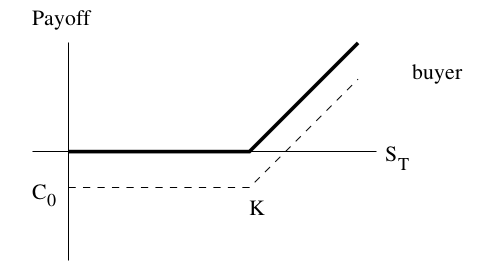
\includegraphics[width=1\linewidth]{Buyer_call} 
		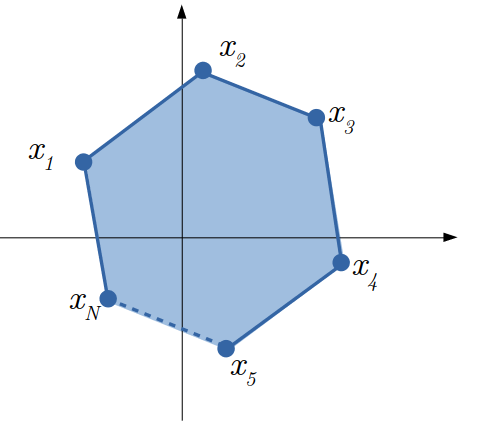
\includegraphics[width=1\linewidth]{Gordan-i*} 
		%\caption{Alternativa $ i*) $.}
		%\label{fig:gordan-i*}
	\end{minipage}
	\begin{minipage}{0.5\textwidth}
		%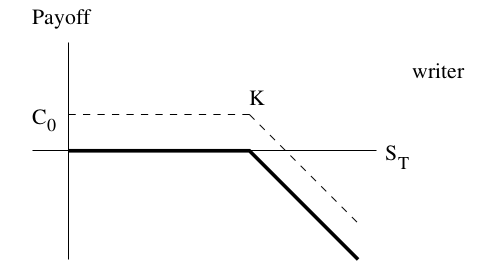
\includegraphics[width=1\linewidth]{Writer_call}
		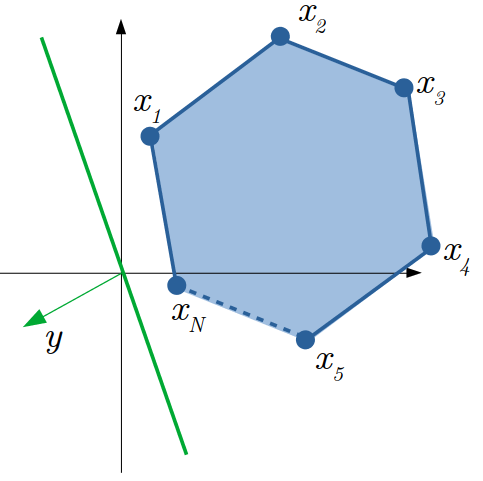
\includegraphics[width=1\linewidth]{Gordan-ii*}
		%\caption{Alternativa $ ii*) $.}
		%\label{fig:gordan-ii*}
	\end{minipage}
	\caption{A la izquierda alternativa $ i^*) $ y a la derecha la alternativa $ ii^*) $.}
	\label{fig:gordan-clasic}
\end{figure}

\bigskip
\begin{teoremaBox}[Teorema de la Alternativa de Gordan-versión convexa]\label{Gordan}
	Sean $ C $ un subconjunto convexo de un espacio vectorial, $ N \in \NN $ y  $ f_1,...,f_N : C \longrightarrow \RR $ funciones convexas. Entonces una, y solo una, de la siguientes afirmaciones se cumple:
	\begin{itemize}
		\item[i)] $ \exists \mathbf{t} \in \Delta_N $ tal que $ 0 \leq \displaystyle \inf_{c\in C}  \sum_{i=1}^{N}{t_i f_i (c)}$.
		\item[ii)] $ \exists c \in C $ que cumple $\displaystyle \max_{i=1\dots,N } f_i(c) < 0 $.
	\end{itemize}
\end{teoremaBox}
\begin{proof}
	Veamos que las alternativas $ i)$ y $ ii) $ son excluyentes y exhaustivas. Para ello, veamos que $ \neg i) \Longleftrightarrow ii) $. Suponemos en primer lugar que el valor de $  \inf_{ c\in C}\left[\max_{i=1\dots,N } f_i(c) \right] \in \RR $.
	
	\begin{itemize}
		\item [$ \Leftarrow $)] Si existe $ c_0 \in C $ tal que $ \max_{i=1\dots,N } f_i(c) < 0 $, entonces, dado $ \ttt \in \Delta_N $,
		\[
		\inf_{ c \in C} \sum_{i=0}^{N}t_i f_i(c) \leq \sum_{i=0}^{N}t_i f_i(c_0) < 0
		\]
		donde la última desigualdad se debe a que $ \ttt \in \Delta_N $. Hemos probado entonces $ \neg i) $.
		\item[$ \Rightarrow $)] 	Si aplicamos el lema de Simons, lema \ref{Simons}, a las funciones $ f_1,...,f_N $ obtenemos:
		
		\begin{equation*}
		\exists t \in \Delta_N \text{ : } \inf_{ c\in C}\left[\max_{i=1\dots,N } f_i(c) \right] = \inf_{c \in C} \sum_{i=1}^{N}t_i f_i (c).
		\end{equation*}
		Entonces, de $ \neg i) $ sabemos que, para este $ \ttt \in \Delta_N $ (como para cualquier otro)
		\[
		\inf_{ c \in C} \sum_{i=0}^{N}t_i f_i(c) < 0
		\]
		luego
		\[
		\inf_{ c\in C}\left[\max_{i=1\dots,N } f_i(c) \right] < 0,
		\]
		como queríamos demostrar.
		
	\end{itemize}
	
	Para finalizar, si $  \inf_{ c\in C}\left[\max_{i=1\dots,N } f_i(c) \right] =-\infty $ es claro que estamos en el caso $ ii) $ y se prueba como en el caso de que dicho ínfimo sea un valor real.
\end{proof}
\bigskip
Destacamos las siguientes observaciones:
\bigskip
\begin{observacion}
	Esta versión convexa del teorema implica la versión clásica del mismo.
\end{observacion}

Para ello, basta aplicar la versión convexa del teorema a $ C := \RR^M $ y a las funciones $ f_1,...,f_N : C \longrightarrow \RR $ definidas por \[ f_i(\ccc):=\langle \ccc, \xx_i \rangle , \forall i=1,...,N.\] Notar que las funciones $ f_1,...,f_N $ son lineales por la izquierda y como consecuencia son convexas. En este caso, la alternativa $ ii) $ implica $ ii*) $ ya que:

\begin{equation*}
\exists \ccc \in C = \RR^M \text{ : } \max_{i=1,...,N} {\langle \ccc,x_i \rangle}  =  \max_{i=1,...,N}f_i (\ccc) < 0 .
\end{equation*}
Por su parte, la alternativa $ i) $ nos da:
\begin{equation*}
\exists \mathbf{t} \in \Delta_N \text{ : } 0 \leq \inf_{\ccc \in \RR^M}  \sum_{i=1}^{N}{t_i f_i(\ccc) } = \inf_{\ccc \in \RR^M} \sum_{i=1}^{N}{t_i\langle \ccc, \xx_i \rangle} = \inf_{\ccc \in \RR^M} \langle \ccc, \sum_{i=1}^{N}{t_i 	\xx_i} \rangle. 
\end{equation*}
Hemos obtenido por ello que  $0  \leq \inf_{\ccc \in \RR^M} \langle \ccc, \sum_{i=1}^{N}{t_i \xx_i} \rangle  $ lo que significa que $ 0 \leq \langle \ccc, \sum_{i=1}^{N}{t_i \xx_i} \rangle  $ para todo $ \ccc \in \RR^M $. Usando la bilinealidad del producto escalar:
\[
0 \leq \langle -\ccc, \sum_{i=1}^{N}{t_i \xx_i} \rangle \Longleftrightarrow 	0 \leq -\langle \ccc, \sum_{i=1}^{N}{t_i \xx_i} \rangle 
\Longleftrightarrow  \langle \ccc, \sum_{i=1}^{N}{t_i \xx_i}\rangle \leq 0, \quad \forall \ccc \in \RR^M.
\]
Juntando ambas desigualdades obtenemos que $ 0 =  \langle \ccc, \sum_{i=1}^{N}{t_i \xx_i}\rangle, \quad \forall \ccc \in \RR^M $. Como la igualdad anterior se cumple para todo elemento de $ \RR^M $ entonces podemos deducir que $ \sum_{i=1}^{N}{t_i \xx_i} = 0 $	ya que $ \sum_{i=1}^{N}{t_i \xx_i} \in (\RR^M)^{\perp} = \{0\} $. Así pues, tenemos que $ i) $ equivale a $ i*) $. \hspace{8.5cm}\qedsymbol 

\bigskip
\begin{observacion}
	El lema de Simons (lema \ref{Simons}) y el teorema convexo de la Alternativa de Gordan (teorema \ref{Gordan}) son equivalentes.
\end{observacion}

\paragraph{} Ya hemos visto que el Lema de Simons implica el Teorema de la Alternativa de Gordan. Veamos que el recíproco también es cierto.  \\

Llamamos $ \alpha := \inf_{ c\in C}\left[\max_{i=1\dots,N } \{f_i(c)\} \right] $. Si $ \alpha = -\infty $. Por el lema \ref{lema2.1} sabemos que $ \forall \ttt \in \Delta_N $ se cumple que $ \sum_{i=1}^{N} t_i f_i(c) \leq \max_{i=1\dots,N } \{f_i(c)\}$ para todo $ c \in C$. Tomando ínfimos en C:
\[
\inf_{c \in C}\left[ \sum_{i=1}^{N} t_i f_i(c) \right] \leq \inf_{ c\in C}\left[\max_{i=1\dots,N } \{f_i(c)\} \right] = -\infty \Longrightarrow \inf_{ c \in C}\left[ \sum_{i=1}^{N} t_i f_i (c)\right] = -\infty 
\]
y por ello $ \forall \ttt \in \Delta_N $ (en particular para uno cualquiera) se cumple que

\[
\inf_{c \in C}\left[ \sum_{i=1}^{N} t_i f_i (c) \right] = \inf_{ c\in C}\left[\max_{i=1\dots,N } \{f_i(c)\} \right]. \]
Supongamos ahora que $ \alpha \in \RR $. Sean las funciones $ g_1, ..., g_N: C \longrightarrow \RR $ definidas como $ g_i = f_i - \alpha $ con $ i=1,...,N$. Veamos que las funciones $ g_1, ..., g_N $ son convexas como consecuencia de que $ f_1, ..., f_N $ lo son. Sean $ i = 1, \dots, N $, $ c_1,c_2 \in C $ y $ \lambda \in \left[0,1\right] $:
\begin{equation*}
\begin{split}
g_i(\lambda c_1 + (1-\lambda) c_2) &= f_i(\lambda c_1 + (1-\lambda) c_2) - \alpha \\
&\leq \lambda f_i(c_1) + (1-\lambda)f_i(c_2) - \alpha \\
&= \lambda f_i(c_1) + (1-\lambda)f_i(c_2) - \lambda \alpha + (1-\lambda)\alpha \\
&= \lambda( f_i(c_1) - \alpha ) + (1-\lambda) (f_i (c_2) - \alpha) \\
&= \lambda g_i(c_1) + (1-\lambda) g_i (c_2).
\end{split}
\end{equation*}
Obtenemos así que $ g_i $ es convexa para todo $ i = 1, ..., N $. Si usamos el Teorema de la Alternativa de Gordan obtenemos que solo se puede dar una y solo de las siguientes posibilidades:

\begin{itemize}
	\item[i)] $ \exists \mathbf{t} \in \Delta_N $ tal que $ 0 \leq \inf_{c \in C}  \sum_{i=1}^{N}{t_i g_i (c)}$.
	\item[ii)] $ \exists c \in C $ que cumple $ \max_{i=1\dots,N } \{g_i(c)\}  < 0 $.
\end{itemize}

Razonemos que no se puede dar $ ii) $. Si fuese así, tendríamos que $ \exists c \in C $ tal que $ \max_{i=1\dots,N } \{g_i(c)\} =  \max_{i=1\dots,N } \{f_i(c) - \alpha \} < 0 $. En particular, se cumpliría \[ f_j(c) - \alpha < 0 \Longrightarrow f_j(c) < \alpha = \inf_{ c\in C}\left[\max_{i=1\dots,N } \{f_i(c)\} \right],\hspace{2mm} \forall  j \in {1,...,N}. \] Esto es imposible por la propia definición de $ \alpha $. Por ello, afirmamos que $ \exists \mathbf{t} \in \Delta_N $ tal que $ 0 \leq \inf_{C}  \sum_{i=1}^{N}{t_i g_i}$. Desarrollando el sumatorio:
\begin{equation*}
\begin{split}
0 &\leq \inf_{c \in C}  \sum_{i=1}^{N}{t_i g_i (c)}\\
 &= \inf_{c \in C}  \sum_{i=1}^{N}{t_i(f_i(c) - \alpha)} \\
&= \inf_{c \in C} \left[ \sum_{i=1}^{N}{t_i f_i(c)} - \sum_{i=1}^{N}{t_i\alpha} \right]\\
&= \inf_{c \in C} \left[ \sum_{i=1}^{N}{t_i f_i(c)} -\alpha \sum_{i=1}^{N}{t_i} \right] \\ 
&= \inf_{c \in C} \left[ \sum_{i=1}^{N}{t_i f_i(c)} - \alpha \right] \\
&= \inf_{c \in C} \left[ \sum_{i=1}^{N}{t_i f_i(c)}\right] - \alpha.
\end{split}
\end{equation*}
Por lo tanto:
\[
0 \leq \inf_{c \in C} \left[ \sum_{i=1}^{N}{t_i f_i(c)}\right] - \alpha \Longleftrightarrow \inf_{c \in C}\left[ \max_{i=1\dots,N } \{f_i(c)\}\right] = \alpha  \leq \inf_{c \in C} \left[ \sum_{i=1}^{N}{t_i f_i(c)}\right].
\]
El lema \ref{lema2.1} nos aporta la otra desigualdad y llegamos nuevamente a que $ \exists \ttt \in \Delta_N $ que cumple:
\[
\inf_{c \in C}\left[ \max_{i=1\dots,N } \{f_i(c)\}\right] = \inf_{c \in C} \left[ \sum_{i=1}^{N}{t_i f_i(c)}\right]. \]
\hspace{12.2cm}\qedsymbol 

\bigskip

Mencionemos antes de terminar que el teorema de la alternativa de Gordan no solo es equivalente al lema de Simons. Otro tipo de teorema de la alternativa equivalente es el lema de Farkas que estudiaremos en el capítulo sobre optimización. Son muchos los teoremas de la alternativa que se conocen, y siempre vinculados a la optimización: véase, por ejemplo, la amplia muestra que aparece recogida en \cite{giorgi2004mathematics}. A modo de ejemplo, y usando la notación clásica matricial, enunciaremos algunos de los resultados más conocidos:

\bigskip
\begin{teoremaBox}[Motzkin]
Dados $ N,M \in \NN $, tomamos las matrices $ A,B,D \in \RR^{M\times N} $. Entonces una, y solo una, de las siguientes condiciones se cumple:
\begin{itemize}
\item[m1)] $ \exists \xx \in \RR^N  $ tal que $ A\xx = 0 $, $ B\xx \geq 0 $ y $ D\xx > 0$.
\item[m2)] $ \exists \yy, \vv, \ww \in \RR^M $ tales que $ \yy^T A + \vv^T B + \ww^T D = 0 $, $ \vv \geq 0 $ y $\ww \geq 0 $.
\end{itemize} 
\end{teoremaBox}
\bigskip

\begin{teoremaBox}[Tucker]
Dados $ N,M \in \NN $, tomamos $ A,B,D \in \RR^{M\times N} $. Entonces una, y solo una, de las siguientes condiciones se cumple:
	\begin{itemize}
		\item[m1)] $ \exists \xx \in \RR^N  $ tal que $ A\xx = 0 $, $ B\xx \geq 0 $ y $ D\xx \geq 0$.
		\item[m2)] $ \exists \yy, \vv, \ww \in \RR^M $ tales que $ \yy^T A + \vv^T B + \ww^T D = 0 $, $ \vv \geq 0 $ y $\ww > 0 $.
	\end{itemize} 
\end{teoremaBox}
\bigskip

\begin{teoremaBox}[Primer teorema de la alternativa de Fenchel]
	Dados $ N,M \in \NN $, tomamos $ A,B \in \RR^{M\times N} $. Entonces una, y solo una, de las siguientes condiciones se cumple:
	\begin{itemize}
		\item[m1)] $ \exists \xx, \zz \in \RR^N  $ tales que $ A\xx + B\zz = 0 $, $ \xx \geq 0 $ y $ \zz \geq 0$.
		\item[m2)] $ \exists \yy \in \RR^M $ tal que $ \yy^T A \geq 0 $ e $ \yy^T B > 0 $.
	\end{itemize} 
\end{teoremaBox}
\bigskip